%% LyX 2.3.7 created this file.  For more info, see http://www.lyx.org/.
%% Do not edit unless you really know what you are doing.
\documentclass[10pt,english,t,10pt]{beamer}
\usepackage{lmodern}
\usepackage[T1]{fontenc}
\usepackage[utf8]{inputenc}
\setcounter{tocdepth}{1}
\setlength{\parskip}{\smallskipamount}
\setlength{\parindent}{0pt}
\usepackage[authoryear]{natbib}

\makeatletter
%%%%%%%%%%%%%%%%%%%%%%%%%%%%%% Textclass specific LaTeX commands.
% this default might be overridden by plain title style
\newcommand\makebeamertitle{\frame{\maketitle}}%
% (ERT) argument for the TOC
\AtBeginDocument{%
  \let\origtableofcontents=\tableofcontents
  \def\tableofcontents{\@ifnextchar[{\origtableofcontents}{\gobbletableofcontents}}
  \def\gobbletableofcontents#1{\origtableofcontents}
}

%%%%%%%%%%%%%%%%%%%%%%%%%%%%%% User specified LaTeX commands.



\usepackage{tikz}
\usetikzlibrary{positioning}
\usepackage{appendixnumberbeamer}

\usepackage{graphicx}
\usepackage{subfig}

\usetheme[progressbar=frametitle,block=fill,subsectionpage=progressbar]{metropolis}

% margin
\setbeamersize{text margin right=1.5cm}

% colors
\definecolor{DarkRed}{rgb}{0.7,0,0}
%\colorlet{DarkRed}{red!70!black}
\setbeamercolor{normal text}{fg=black}
\setbeamercolor{alerted text}{fg=DarkRed}
\setbeamercolor{progress bar}{fg=DarkRed}
\setbeamercolor{button}{bg=DarkRed}

% width of seperators
\makeatletter
\setlength{\metropolis@titleseparator@linewidth}{1pt}
\setlength{\metropolis@progressonsectionpage@linewidth}{1pt}
\setlength{\metropolis@progressinheadfoot@linewidth}{1pt}
\makeatother

% new alert block
\newlength\origleftmargini
\setlength\origleftmargini\leftmargini
\setbeamertemplate{itemize/enumerate body begin}{\setlength{\leftmargini}{4mm}}
\let\oldalertblock\alertblock
\let\oldendalertblock\endalertblock
\def\alertblock{\begingroup \setbeamertemplate{itemize/enumerate body begin}{\setlength{\leftmargini}{\origleftmargini}} \oldalertblock}
\def\endalertblock{\oldendalertblock \endgroup}
\setbeamertemplate{mini frame}{}
\setbeamertemplate{mini frame in current section}{}
\setbeamertemplate{mini frame in current subsection}{}
\setbeamercolor{section in head/foot}{fg=normal text.bg, bg=structure.fg}
\setbeamercolor{subsection in head/foot}{fg=normal text.bg, bg=structure.fg}

% footer
\makeatletter
\setbeamertemplate{footline}{%
    \begin{beamercolorbox}[colsep=1.5pt]{upper separation line head}
    \end{beamercolorbox}
    \begin{beamercolorbox}{section in head/foot}
      \vskip1pt\insertsectionnavigationhorizontal{\paperwidth}{}{\hskip0pt plus1filll \insertframenumber{} / \inserttotalframenumber \hskip2pt}\vskip3pt% 
    \end{beamercolorbox}%
    \begin{beamercolorbox}[colsep=1.5pt]{lower separation line head}
    \end{beamercolorbox}
}
\makeatother

% toc
\setbeamertemplate{section in toc}{\hspace*{1em}\inserttocsectionnumber.~\inserttocsection\par}
\setbeamertemplate{subsection in toc}{\hspace*{2em}\inserttocsectionnumber.\inserttocsubsectionnumber.~\inserttocsubsection\par}



% code
\usepackage{xcolor}
\usepackage{listings}

\definecolor{codegray}{rgb}{0.5,0.5,0.5}
\definecolor{background}{HTML}{F5F5F5}
\definecolor{keyword}{HTML}{4B69C6}
\definecolor{string}{HTML}{448C27}
\definecolor{comment}{HTML}{448C27}

\usepackage{inconsolata}
\lstdefinestyle{mystyle}{
    commentstyle=\color{comment},
    keywordstyle=\color{keyword},
    stringstyle=\color{string},
    basicstyle=\ttfamily,
    breakatwhitespace=false,         
    breaklines=true,                 
    captionpos=b,                    
    keepspaces=true,                                    
    numbersep=5pt,                  
    showspaces=false,                
    showstringspaces=false,
    showtabs=false,
    tabsize=4,
	showlines=true
}

\lstset{style=mystyle}

\makeatother

\usepackage{babel}
\begin{document}
\title{14b. Exam + Q\&A\vspace{-2mm}}
\subtitle{Adv. Macro: Heterogenous Agent Models} 
\author{Nicolai Waldstrøm}
\date{2024}

{
\setbeamertemplate{footline}{} 
\begin{frame}

\maketitle

\begin{tikzpicture}[overlay, remember picture]
\node[above left=0cm and 0.0cm of current page.south east] 
{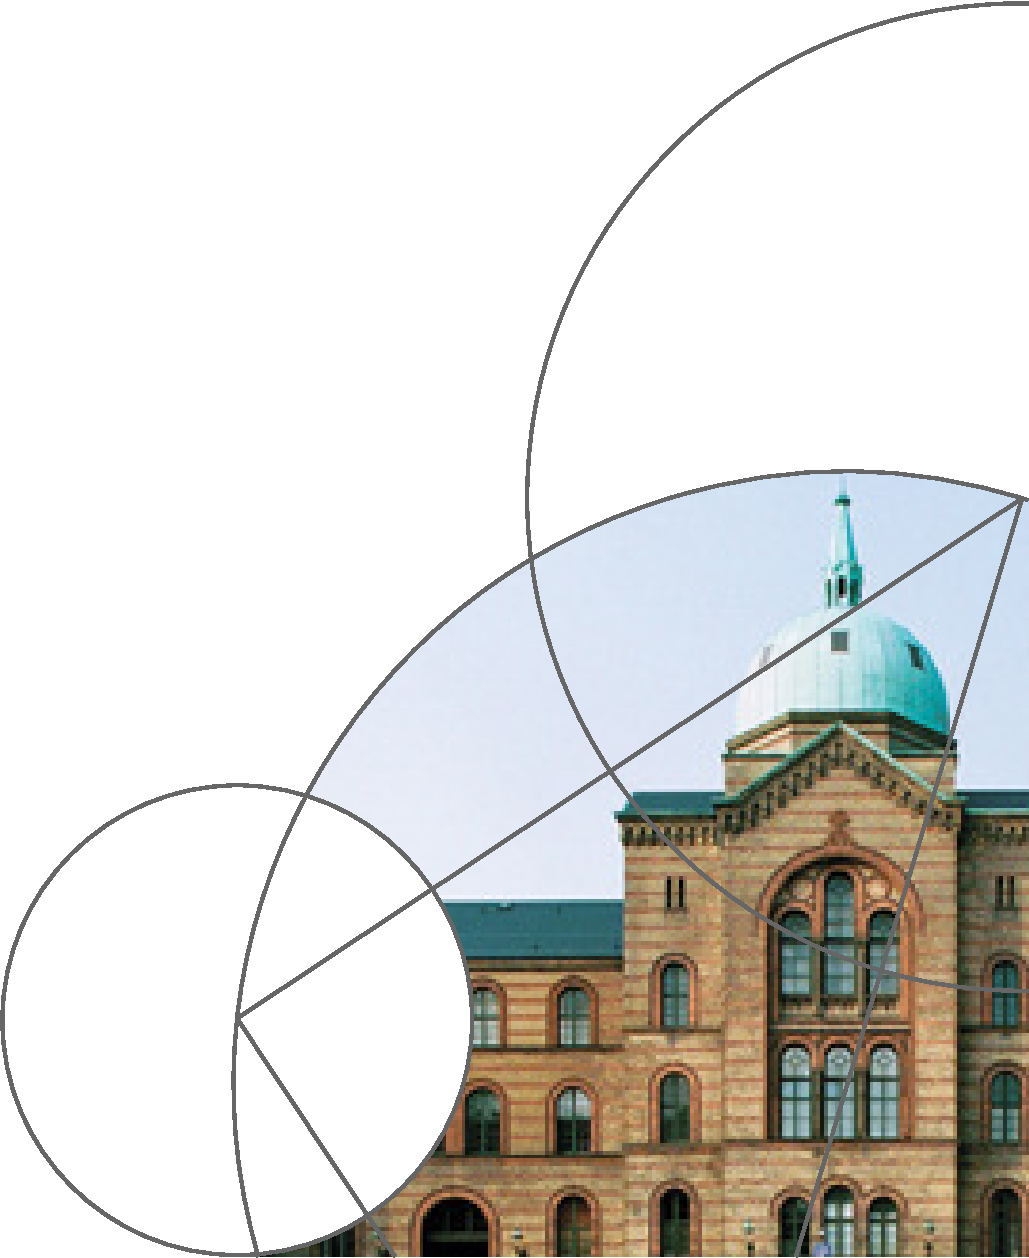
\includegraphics[width=4cm]{figs/KUSAMFtitlelrcorner.pdf}};
\end{tikzpicture}

\begin{tikzpicture}[overlay, remember picture]
\node[below left=0.5cm and .8cm of current page.north east] 
{\includegraphics[width=1.5cm]{figs/KUSAMFlogo.pdf}};
\end{tikzpicture}


\end{frame}
}

\addtocounter{framenumber}{-1}

\section{Exam}

\begin{frame}{Exam info}
\begin{itemize}
\item <+->Portfolio part:
\begin{itemize}
\item Ensure that assignments are in good shape 
\item \textbf{Use the feedback you have received}!
\end{itemize}
\item <+->Take-home part:
\begin{itemize}
\item 36-hour take home
\begin{itemize}
\item Solveable in 24 hours (hopefully less)
\end{itemize}
\item \textbf{Will not feature any significant coding }
\item Focus on how to solve and analyze model using GEModelTools
\item Analyze results using intuition from the lectures
\end{itemize}
\end{itemize}
\end{frame}
%
\begin{frame}{Preparation for exam}
\begin{itemize}
\item <+->Go through lecture slides + course plan 
\begin{itemize}
\item <+->Ensure that you have a good understanding of the various models 
\item <+->Buffer-stock model, HANC, NK, HANK, HANK-SAM, IHANK etc.
\end{itemize}
\item <+->\textbf{Redo exercises} - check with solutions in the github
repo 
\item <+->Ensure that you are comfortable with GEModelTools
\begin{itemize}
\item <+->Steady state (model.find\_ss() $\Rightarrow$\textrm{ }model.ss)
\item <+->Jacobians (model.\_compute\_jac\_hh() $\Rightarrow$ model.jac\_hh,
model.compute\_jacs() $\Rightarrow$ model.jac)
\item <+->Linear transition path (model.find\_IRFs() $\Rightarrow$ model.IRF{[}'x'{]})
\item <+->Non-linear transition path (model.find\_transition\_path() $\Rightarrow$
model.path.x)
\end{itemize}
\item <+->Troubleshooting in GEModelTools
\begin{itemize}
\item <+->Check examples in notebook repo (github.com/NumEconCopenhagen/GEModelToolsNotebooks)
\item <+->Check documentation or \textbf{source code}
\end{itemize}
\end{itemize}
\end{frame}
%
\begin{frame}{Q\&A I}
\begin{itemize}
\item <+->\emph{\small{}What was the motivation for linearization in Lecture
8? Was it to show that linearization to a first-order approximation
gives the same result as aggregated uncertainty?}{\small\par}
\begin{itemize}
\item <+->{\small{}Consider a model A without aggregate uncertainty and
model B with aggregate uncertainty. If we linearize (i.e. do a first-order
approximation) w.r.t aggregate shocks, the impulse responses to the
two models are the }\textbf{\small{}same}{\small{}. }{\small\par}
\end{itemize}
\item <+->\emph{\small{}In the last lecture (Lecture 12), Jeppe used the
decompose function in GEModelTools. What was the reason it couldn't
be used in exercises for Lecture 11? And does it have something to
do with linearization? }{\small\par}
\begin{itemize}
\item <+->{\small{}Yes, the build in decompose function in GEModelTools
(decompose\_hh\_}\textbf{\small{}path}{\small{}) only-works with non-linear
solution (find\_transition\_path()). It would be easy to write a similar
function decompose using the linear solution to the model, but currently
it is not there. }{\small\par}
\end{itemize}
\end{itemize}
\end{frame}
%
\begin{frame}{Q\&A II}
\begin{itemize}
\item <+->\emph{What is the difference between the model with aggregate
uncertainty and models that only include idiosyncratic uncertainty?
More specifically, how do I identify aggregate uncertainty in a model,
and what are the implications of having aggregate uncertainty?}
\begin{itemize}
\item <+->No aggregate uncertainty = perfect foresight. No expectations
w.r.t aggregate variables ($w_{t+1},r_{t+1}$ etc.), only w.r.t micro
level het. ($e_{it+1}$)
\item <+->Aggregate uncertainty $\Rightarrow$ The value of aggregate shocks
is unknown next period $\Rightarrow$ Next-period endo. variables
$w_{t+1},r_{t+1}$ are uncertain
\end{itemize}
\item <+->Implications of aggregate uncertainty:
\begin{itemize}
\item Precautionary behavior w.r.t aggregates $w,r$
\item Non-linear business cycle simulation (ZLB etc.)
\item Needed to study large, once-in-a-lifetime shocks (e.g. financial crisis)
\end{itemize}
\end{itemize}
\end{frame}
%
\begin{frame}{Q\&A III}
\begin{itemize}
\item <+->\textbf{Q:} \emph{In the literature, HANC is also referred to
as the Standard Incomplete Market (SIM) model. I find it difficult
to understand the concept of “incomplete markets.” Does it simply
mean that risk is uninsurable such that agents instead must create
a buffer by accumulating assets?}
\item <+->\textbf{A}: Consider a simple HH problem with two individuals
$A,B$ where idiosynchratic income $e_{i}$ takes two values $[0,1]$
and with $Ee_{i}=0.5$. With \emph{complete insurance markets }it
is possible for agents to enter a state-contigent contract which fully
insures against any risk:
\begin{itemize}
\item Bond 1 $B_{1}$ pays 1 in state $e_{A}=0$ and 0 if $e_{A}=1$
\item Bond 2 $B_{2}$ pays 0 in state $e_{A}=1$ and 1 if $e_{A}=0$
\end{itemize}
\item <+->If agents are risk aversion utility maximization will imply that
$A$ and $B$ exactly buy and trade bonds such that they perfectly
insure \textbf{each other }against risk
\begin{itemize}
\item $A$ buys enough of bond $B_{1}$ so that when she is in a bad state
she is compensated for the earnings loss buy $B$, and vice versa.
Both $A,B$ end up with exactly the same income and wealth ex-post.
\end{itemize}
\item <+->The assumption of incomplete markets imply that state-contigent
claims ($B_{1},B_{2}$) does not exist. 
\end{itemize}
\end{frame}
%
\begin{frame}{Q\&A IIII}
\begin{itemize}
\item <+->\emph{What are your tips for writing about het-agent models for
a master’s thesis?}
\begin{itemize}
\item <+->Find a research question that interests you 
\begin{itemize}
\item Not specific to MA in het-agent macro
\end{itemize}
\item <+->Find a paper that is closely related to the topic
\end{itemize}
\item <+->Prioritize finding a topic which is closely related to what we
have seen in this course
\begin{itemize}
\item This enables you to start from the code you have been given in this
course
\item (or can find in GEModelToolsNotebooks)
\end{itemize}
\item <+->Example:
\begin{itemize}
\item <+->\textbf{Q}: Does automatic stabalizers reduce cyclical inequality?
\item <+->\textbf{Paper}: McKay \& Reis (2016) >>The role of automatic
stabilizers in the US business cycle<<
\item <+->\textbf{Build on}: Basic HANK (lecture 9) or HANK-SAM (lecture
12)
\end{itemize}
\end{itemize}
\end{frame}
%

\end{document}
